Para o projeto do controlador utilizamos uma estrutura \gls{pid} na forma
paralela com os valores sintonizados a partir do ensaio ao degrau de
Ziegler-Nichols utilizando a planta do sensor 1 pela \Eqref{planta-sensor-1-zn}
em tempo contínuo, de acordo com a \Eqref{controlador-pid-paralelo}:

\begin{equation}
  \eqlabel{controlador-pid-paralelo}
  C_{\mathrm{pid}}(s) = 9.53 + \frac{0.043}{s} + \frac{583s}{s+100}
\end{equation}

Apesar do \gls{pid} ter demonstrado boa estabilidade, rapidez na resposta e
rejeição a perturbações, ainda havia um \gls{ess} considerável ao tentar
acompanhar a curva de referência, principalmente no início da dinâmica com a
rampa. 

Para melhorar esse desempenho optamos por adotar uma segunda estrutura de
\gls{ff} utilizando o modelo inverso da planta da \Eqref{planta-sensor-1-zn} em
paralelo com o \gls{pid}, juntamente com um filtro passa-baixas para garantir
causalidade, resultando na \Eqref{controlador-ff}. Dessa forma, conseguimos
antecipar a ação de controle necessária para obter um melhor acompanhamento da
referência.

\begin{equation}
  \eqlabel{controlador-ff}
  C_{\mathrm{ff}} = \frac{188.0271s + 1}{92 s + 0.92}
\end{equation}

A estrutura completa do controlador é apresentada na \Figref{bloco-controlador}.
Nessa configuração, a ação do \gls{ff} atua diretamente sobre a referência,
enquanto a ação do \gls{pid} é responsável pela correção baseada na
realimentação do sistema.

\begin{figure}[H]
\centering
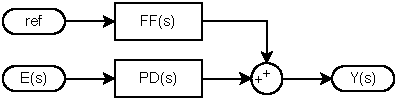
\includegraphics[width=1\linewidth]{images/Bloco Controlador.pdf}
\caption{Estrutura do controlador proposto, composta por uma ação \gls{ff}
aplicada à referência e uma ação \gls{pid} baseada na realimentação do sistema.}
\figlabel{bloco-controlador}
\end{figure}

Para a discretização do controlador utilizamos o método de Tustin para ambas as
ações de controle do \gls{pid} e \gls{ff}. 